\documentclass{standalone}

\usepackage{tikz}
\usepackage{stmaryrd}
\usepackage{amsmath}
\usepackage{amssymb}

\begin{document}

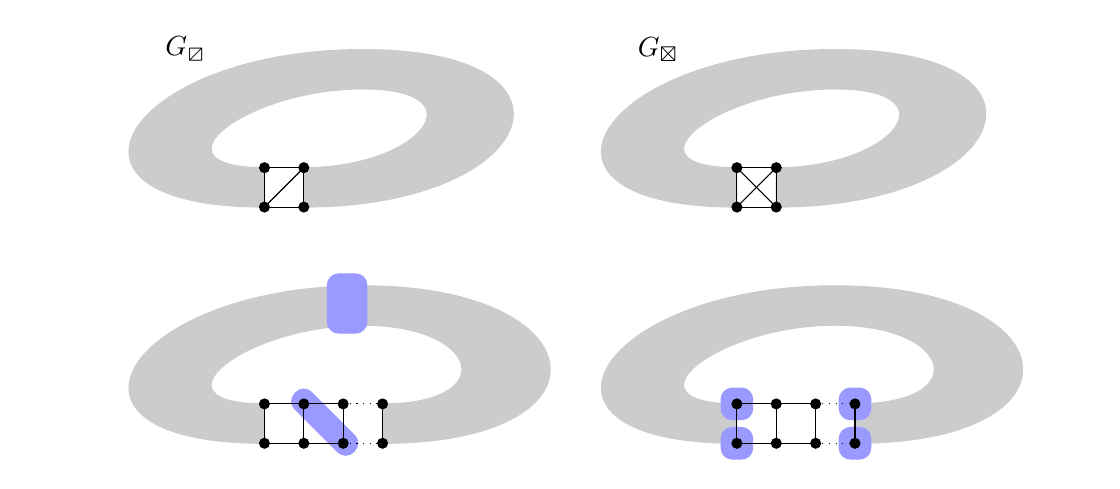
\begin{tikzpicture}

\filldraw[black!20!white] (0,0) .. controls +(-3,0) and +(-3,0) .. (1.25,2) .. controls +(3,0) and +(3,0) .. (.5,0) -- (.5,0.5) .. controls +(1.5,0) and +(1.5,0) .. (1.25,1.5) .. controls +(-1.5,0) and +(-1.5,0) .. (0,0.5) -- cycle;

\fill (0,0) circle (2pt); 
\fill (0,.5) circle (2pt); 
\fill (.5,0) circle (2pt); 
\fill (.5,.5) circle (2pt);

\draw (0,0) -- (0,0.5) -- (0.5,0.5) -- (0.5,0) -- (0,0);
\draw (0.5,0.5) -- (0,0.);

\node at (-1,2) {$G_\boxslash$};

    \begin{scope}[shift={(6,0)}]
\filldraw[black!20!white] (0,0) .. controls +(-3,0) and +(-3,0) .. (1.25,2) .. controls +(3,0) and +(3,0) .. (.5,0) -- (.5,0.5) .. controls +(1.5,0) and +(1.5,0) .. (1.25,1.5) .. controls +(-1.5,0) and +(-1.5,0) .. (0,0.5) -- cycle;

\fill (0,0) circle (2pt); 
\fill (0,.5) circle (2pt); 
\fill (.5,0) circle (2pt); 
\fill (.5,.5) circle (2pt);

\draw (0,0) -- (0,0.5) -- (0.5,0.5) -- (0.5,0) -- (0,0);
\draw (0.5,0.5) -- (0,0.);
\draw (0.5,0) -- (0,0.5);

\node at (-1,2) {$G_\boxtimes$};

\end{scope}

\begin{scope}[shift={(0,-3)}]
\draw[rounded corners, fill, blue!40!white, rotate around={-45:(0.5,0.25)}] (0.15,0.30) rectangle (1.2,0.6) ;
\filldraw[black!20!white] (0,0) .. controls +(-3,0) and +(-3,0) .. (1.25,2) .. controls +(3,0) and +(3,0) .. (1.5,0) -- (1.5,0.5) .. controls +(1.5,0) and +(1.5,0) .. (1.25,1.5) .. controls +(-1.5,0) and +(-1.5,0) .. (0,0.5) -- cycle;

\draw[rounded corners, fill, blue!40!white, rotate around={-90:(1.25,1.75)}] (0.85,1.30) rectangle (1.6,1.8) ;
\fill (0,0) circle (2pt);
\fill (0,.5) circle (2pt);
\fill (.5,0) circle (2pt);
\fill (.5,.5) circle (2pt);
\fill (1,0) circle (2pt);
\fill (1,0.5) circle (2pt);
\fill (1.5,0) circle (2pt);
\fill (1.5,0.5) circle (2pt);

\draw (0,0) -- (0,0.5) -- (0.5,0.5) -- (0.5,0) -- (0,0);
\draw (0.5,0.5) -- (1,0.5) -- (1,0) -- (0.5,0) -- (0.5,0.5);
\draw (1.5,0) -- (1.5,.5);

\draw[dotted] (1,0) -- (1.5,0);
\draw[dotted] (1,0.5) -- (1.5,0.5);

\end{scope}

    \begin{scope}[shift={(6,-3)}]

\filldraw[black!20!white] (0,0) .. controls +(-3,0) and +(-3,0) .. (1.25,2) .. controls +(3,0) and +(3,0) .. (1.5,0) -- (1.5,0.5) .. controls +(1.5,0) and +(1.5,0) .. (1.25,1.5) .. controls +(-1.5,0) and +(-1.5,0) .. (0,0.5) -- cycle;


\def\shift{0.2}

\draw[rounded corners, fill, blue!40!white] (-\shift,-\shift) rectangle (\shift,\shift);
\draw[rounded corners, fill, blue!40!white] (1.5-\shift,-\shift) rectangle (1.5+\shift,\shift);
\draw[rounded corners, fill, blue!40!white] (1.5-\shift,0.5-\shift) rectangle (1.5+\shift,0.5+\shift);
        \draw[rounded corners, fill, blue!40!white] (-\shift,0.5-\shift) rectangle (\shift,0.5+\shift);
\fill (0,0) circle (2pt);
\fill (0,.5) circle (2pt);
\fill (.5,0) circle (2pt);
\fill (.5,.5) circle (2pt);
\fill (1,0) circle (2pt);
\fill (1,0.5) circle (2pt);
\fill (1.5,0) circle (2pt);
\fill (1.5,0.5) circle (2pt);

\draw (0,0) -- (0,0.5) -- (0.5,0.5) -- (0.5,0) -- (0,0);
\draw (0.5,0.5) -- (1,0.5) -- (1,0) -- (0.5,0) -- (0.5,0.5);
\draw (1.5,0) -- (1.5,.5);

\draw[dotted] (1,0) -- (1.5,0);
\draw[dotted] (1,0.5) -- (1.5,0.5);


\end{scope}

\end{tikzpicture}

\end{document}
